%!TEX root = ../lectionsA4.tex

\epigraph{\textit{"<Ежели спросят у Вас: что важнее – Солнце или Луна, ответствуйте – Луна. Ибо Солнце светит днем, когда и без того светло, а Луна – ночью">} \\ Козьма Прутков}

\section{Виды и значение калибровок для апертурного синтеза}
Калибровка - одна из самых значимых составляющих наблюдений на радиоинтерферометрах, потому что без них не удастся построить изображение. По данным, не включающим калибровки, можно оценивать лишь некоторые интегральные параметры излучения, например, получить корреляционные кривые, но даже для их правильной интерпретации также необходимо проведение калибровок.

\subsection{Виды калибровок}
Калибровки бывают аппаратные (до наблюдений) и применительно к данным. Аппаратные калибровки чрезвычайно важны, так как после проведения наблюдений нейтрализовать их негативное воздействие практически невозможно\\

\begin{list}{-}{\textbf{Аппаратные}}
	\item \textit{Наведение антенн} \\
	Так как диаграмма направленности антенны с круглой апертурой является функцией Бесселя, и данная функция имеет один выраженный максимум, то он должен смотреть точно на центр солнечного диска. При ошибке наведения возникает наклон (см. рис. \ref{fig:искажения при наведении}), который приводит к неправильной фокусировке облучателя и довольно сложным искажениям как фазы, так и амплитуды. Поэтому необходимо следить за точностью движения моторов и их способностью выдерживать определенные эфимериды, а также за положением облучателя антенны
	\begin{figure}[H]
		\centering
		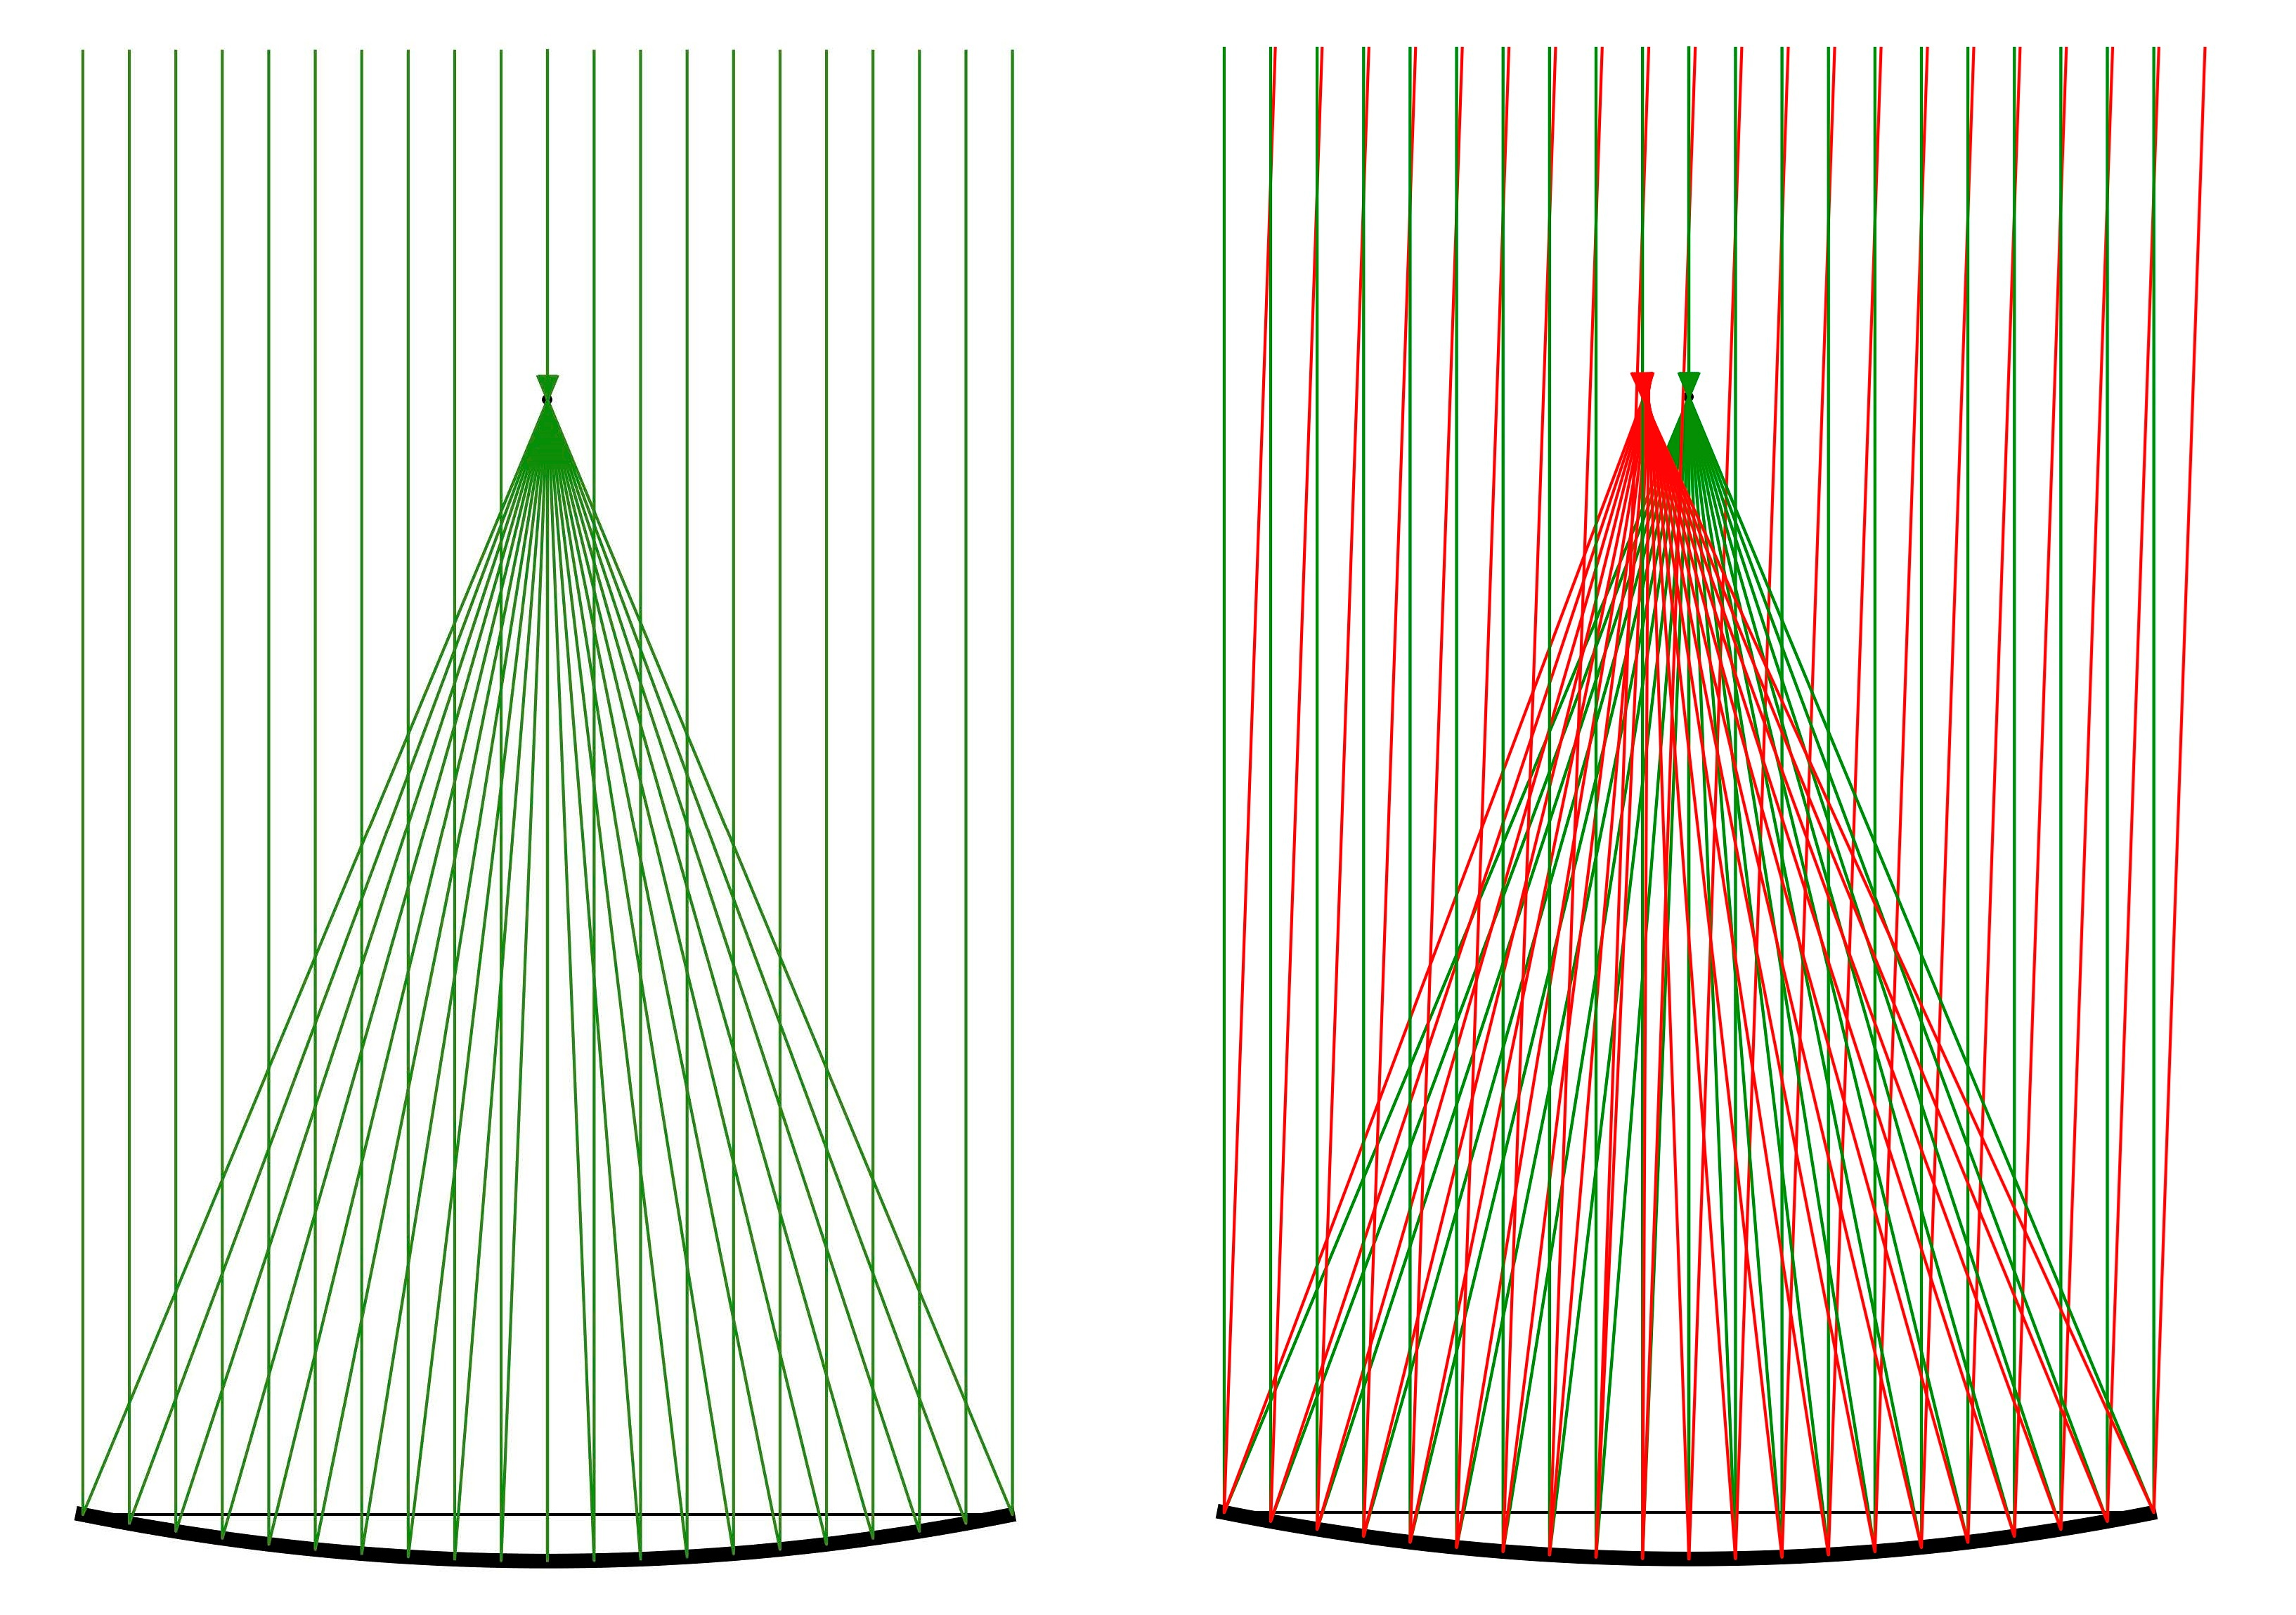
\includegraphics[scale=0.15]{images/globa2.jpg}
		\caption{Ошибки фокусировки при неправильном наведении}
		\label{fig:искажения при наведении}
	\end{figure}

	\item \textit{Положение антенн относительно друг друга}\\ (можно оценить из данных наблюдений и изменить с помощью подстроечных болтов на стойках)

	\textbf{20-30 мин доделать}

	\item \textit{Длины кабелей и идентичность их физических параметров}\\
	На каждой антенне есть приемный модуль, в котором установлен лазер. Он используется для передачи модулированного сигнала по оптоволокну к коррелятору. Однако, если длины кабелей будут различны, то возникнут дополнительные фазовые искажения. Например, различие длин в 1 см даст 36 градусов фазового набега на частоте 3 ГГц.\\
	Для того чтобы этого не допустить, все кабели имеют одинаковую длину в 800 метров, вне зависимости от положения антенн относительно блока коррелятора, и накручены на так называемые "<компенсационные катушки">. Измеряются длины с ограниченной ($\approx 1$ метр) точностью прибором под названием "<рефлектометр">, при этом происходит измерение именно оптической длины, так как электрическая и геометрическая длины оптических кабелей различаются.\\
	Однако есть возможность уточнить измеренную величину с точностью до нескольких миллиметров путем анализа данных наблюдений и поиска линейных наклонов фаз в полосе частот. Эти небольшие отклонения легче компенсировать программными задержками\\
	Также необходимо учитывать, что температурные колебания влияют на абсолютные значения коэффициентов преломления ядра и оптической оболочки оптоволокна, а следовательно, может меняться скорость света внутри кабеля. Для нейтрализации этого эффекта все коммуникации проложены в подземном тоннеле, где круглогодично поддерживается примерно одинаковая температура.

	\item \textit{Точные координаты, временная привязка, стандарт частоты}\\
	Данные величины необходимо знать с максимально возможной точностью для введения задержек в сигнал с целью фазовых корректировок и остановки вращения интерференционных лепестков (возникает из-за относительного движения источника относительно интерферометра, вызванного вращением Земли). \\
	Скорость вращения лепестков пропорциональна $2\pi \nu_{LO} \tau_g$, где $\nu_{LO}$ - частота гетеродина, $\tau_g = ({D}/{c}) * sin \theta$ - геометрическая задержка (рис. \ref{fig:геометрия интерферометра}).
	\begin{figure}[H]
		\centering
		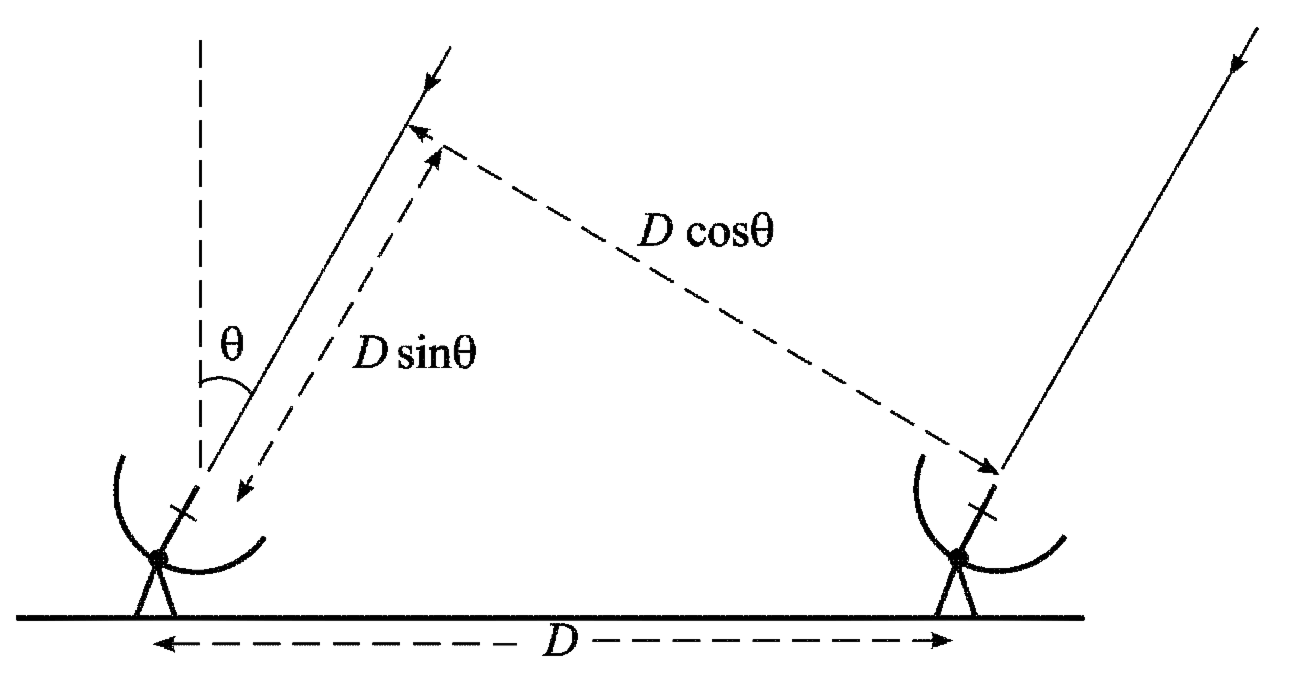
\includegraphics[scale=0.5]{images/geominterferometr.png}
		\caption{Геометрия простого интерферометра. $D$ — база интерферометра}
		\label{fig:геометрия интерферометра}
	\end{figure}

\end{list}

\begin{list}{-}{\textbf{Калибровка данных}}
	\item \textit{Комплексные коэффициенты передачи антенн (antenna-based)}\\
	Под калибровкой данных подразумевается вычисление коэффициентов передачи антенн с использованием данных наблюдений.\\\\
	Методы калибровок данных:
	\begin{itemize}
		\item По наблюдениям точечных источников и известным потоком в полосе частот наблюдений вблизи интересующего объекта (используется преимущественно на звездных радиоинтерферометрах)
		\item С использованием избыточности антенной решетки (много одинаковых пар антенн, измеряющих один и тот же сигнал)
		\item Самокалибровка
	\end{itemize}

	\item ошибки видностей (baseline-based)
\end{list}

\subsection{Самокалибровка}
Самокалибровка производится по наблюдаемому источнику и подразумевает наличие модельного распределения яркости $\hat{I}$, из которого вычисляются модельные видности для каждой пары антенн.

Изначально метод был разработан для того случая, когда общая калибровка проходит по известному объекту, однако он находится в стороне от объекта наблюдения, и при перенаведении телескопа несколько меняется фаза принимаемого сигнала (применять калибровку на одни координаты к другим - в общем случае нельзя). Самокалибровка позволяет вычислить небольшие отклонения и поправки из-за этой смены координат.

Данный метод позволяет получить радиоизображение высокого качества, с динамическим диапазоном порядка $>1000$. Однако для применения самокалибровки необходимо иметь хорошую модель источника, и получить ее -- задача довольно сложная, особенно если учесть высокое разрешение СРГ и необходимость высокой детализации этой модели.

Комплексные коэффициенты передачи антенн при самокалибровке вычисляются путем минимизации функции:
\begin{equation}\label{eq:самокалибровка}
	S = \sum_{k}^{} \sum_{i,j (i \not= j)}^{} \omega_{ij}(t_{k}) \lvert \widetilde{V}_{ij}(t_k) -  g_i(t_k)g_j^*(t_k)\hat{V}_{ij}(t_k) \rvert^2
\end{equation}
где $ \omega_{ij}$ - весовой коэффициент для видности, измеряемой парой антенн $i$ и $j$.\\

Уточнение модели происходит итеративно. Шаги на одной итерации:
\begin{enumerate}
	\item Подобрать модель распределения яркости на небе
	\item Вычислить модельные видности и, подставив их в выражение (\ref{eq:самокалибровка}), найти коэффициенты передачи антенн
	\item Скорректировать измеренные видности на коэффициенты передачи и построить изображения, используя какой-либо метод чистки
	\item Использовать компоненты модели, получаемой при чистке, в качестве нового модельного распределения яркости.
	\item Если результат неудовлетворителен, вернуться к шагу 2.
\end{enumerate}

Метод хорошо применяется к точечным источникам, так как их модельные видности хорошо известны.

\subsection{Калибровка по избыточности}
Данный метод возможно использовать, не зная об источнике абсолютно ничего. Единственное условие применимости данного метода - SNR (отношение сигнал/шум) для каждой видности должно быть $5$ или более. Решение можно найти с точностью до линейного наклона фаз и константы по амплитуде, что
приводит к произвольному положению Солнца в кадре и произвольной яркостной температуре. Эти
эффекты корректируются дополнительными методами.

\begin{figure}[H]
	\centering
	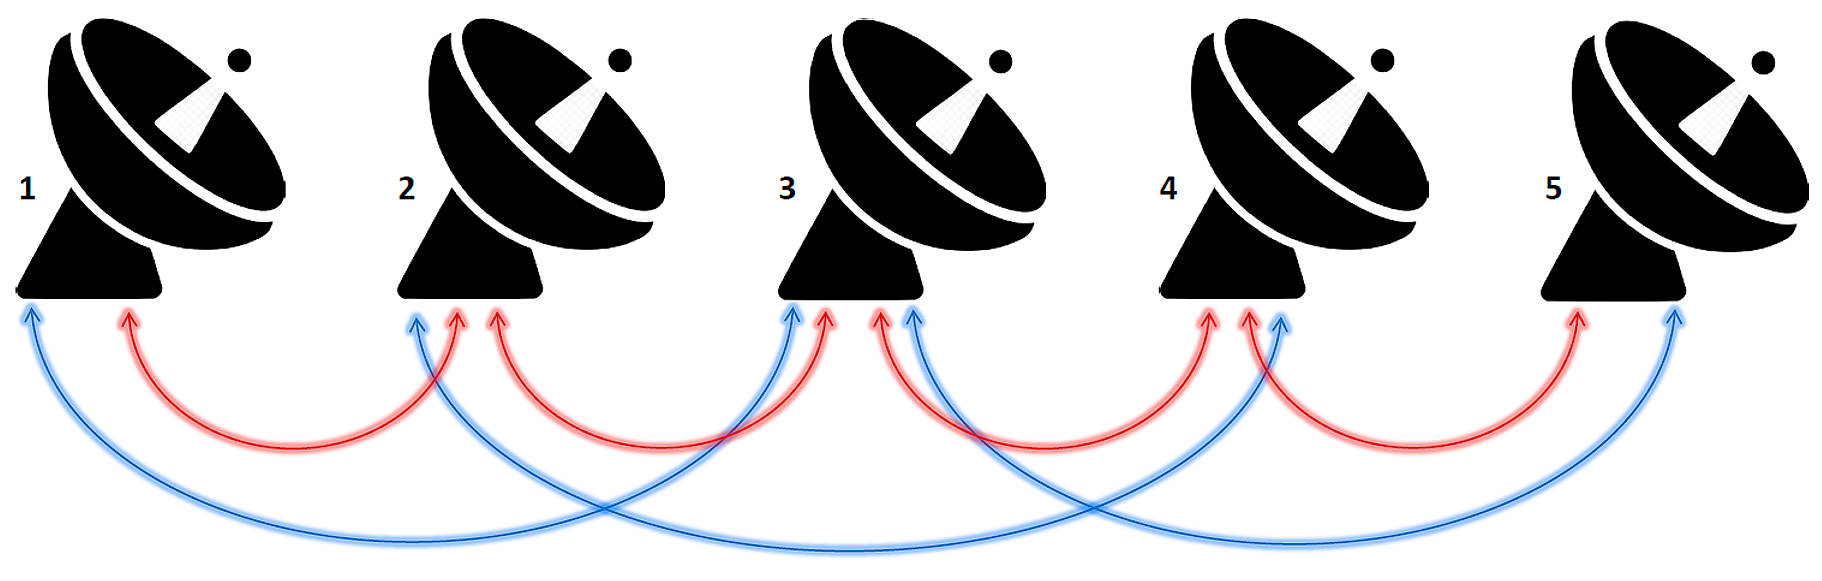
\includegraphics[scale=0.35]{images/calibrate_cheme.png}
	\caption{Схема составления пар антенн для калибровки по избыточности}
	\label{fig:калибровка по избыточности}
\end{figure}

Для построения изображения используются перекрестные базы, а для калибровки - избыточные базы между антеннами одного луча. Если при калибровке использовать только короткие базы, этого будет достаточно для фазовой калибровки, но недостаточно для амплитудной, так как это приводит к появлению артефактов (см. рис. \ref{fig:temp_calib}) -- поэтому необходимо использовать также и длинные избыточные базы.

Итак, нам необходимо решить систему уравнений вида
\begin{equation}\label{eq:калибровка по избыточности 1}
	\widetilde{V}_{kl} = g_kg_l^*V_{kl}
\end{equation}
Как можно заметить из рис. \ref{fig:калибровка по избыточности}, видности на некоторых парах антенн у нас повторяются, а именно:\\
\begin{equation}\label{eq:повторы баз 1}
	V_1 = V_{13} = V_{24} = V_{35}
\end{equation}
\begin{equation}\label{eq:повторы баз 2}
	V_2 = V_{12} = V_{23} = V_{34} = V_{45}
\end{equation}

Аналитически эту систему уравнений решить невозможно, так как все величины комплексные, а уравнения нелинейные. Так как линеаризация этой системы также довольно сложна, решается система численно методами нелинейной минимизации.

Однако покажем, как можно линеаризовать эту систему методом взятия логарифма. \\
Представим ${V}_{kl}(t)$ и ${g}_{k}(t)$ как комплексные числа, перенеся амплитуды под экспоненту:
\begin{equation}\label{eq:замена видности}
	{V}_{kl}(t) = \exp({S}_{kl} + i\psi_{kl}(t))
\end{equation}
\begin{equation}\label{eq:замена коэф передачи}
	{g}_{k}(t) = \exp({a}_{k} + i\phi_{k}(t))
\end{equation}
Подставим замену в изначальное уравнение (\ref{eq:калибровка по избыточности 1}) и возьмем от получившегося выражения логарифм:
\begin{equation}\label{eq:подстановка в 1.2}
	\tilde{S}_{kl}(t) + i\tilde{\psi}_{kl}(t) = {a}_{k}(t) + {a}_{l}(t) + {S}_{kl}(t) + i (\phi_{k}(t) + \phi_{l}(t) + {\psi}_{kl}(t))
\end{equation}
Можно разделить уравнения для фаз и амплитуд:
\begin{equation}\label{eq:разделение для амплитуд}
	\tilde{\psi}_{kl}(t) = \phi_{k}(t) + \phi_{l}(t) + {\psi}_{kl}(t)
\end{equation}
\begin{equation}\label{eq:разделение для фаз}
	\tilde{S}_{kl}(t) = {a}_{k}(t) + {a}_{l}(t) + {S}_{kl}(t)
\end{equation}

\begin{equation}
	\mqty( % It's require package "physics"
	1&-1&0&0&1\\	0&1&-1&0&1\\	0&0&1&-1&1\\	1&0&0&-1&1
	)
	\mqty(
	\phi_{1}\\	\phi_{2}\\	\phi_{3}\\	\phi_{4}\\	\phi_{5}\\	\psi
	)=
	\mqty(
	\tilde{\psi}_{12}\\	\tilde{\psi}_{23}\\	\tilde{\psi}_{34}\\	\tilde{\psi}_{45}
	)
\end{equation}

Когда система недоопределена, у нее всегда есть вектор, принадлежащий нулевому пространству матрицы. Это вектор, который при умножении матрицы на него дает 0. Если

\begin{equation}
	\mqty(
	\phi_{1}\\	\phi_{2}\\	\phi_{3}\\	\phi_{4}\\	\phi_{5}\\	\psi
	)=
	C_1	\mqty(
	1\\	1\\	1\\	1\\	1\\	0\\
	)+
	C_2	\mqty(
	1\\	2\\	3\\	4\\	5\\	0\\
	)
\end{equation}

Система уравнений недоопределена, поэтому имеет бесконечное множестворешений, отличающихся на вектора нулевого пространства матрицы:

\begin{equation}
	\mqty(
	\phi_{1} - \phi_{2} + \phi = \tilde{\psi}_{12}\\
	\phi_{2} - \phi_{3} + \phi = \tilde{\psi}_{23}\\
	\phi_{3} - \phi_{4} + \phi = \tilde{\psi}_{34}\\
	\phi_{4} - \phi_{5} + \phi = \tilde{\psi}_{45}
	)
\end{equation}

Добавление новых уравнений в систему (для более длинных баз) не меняет вид векторов нулевого пространства

\begin{equation}
	\mqty(
	1&-1&0&0&0&1\\	1&-1&0&0&0&1\\	0&1&-1&0&0&1\\	-1&0&0&1&0&1\\ 0&0&1&-1&0&1\\ 1&0&0&0&-1&1
	)
	\mqty(
	\phi_{1}\\	\phi_{2}\\	\phi_{3}\\	\phi_{4}\\	\phi_{5}\\	\psi_1\\ \psi_2
	)=
	\mqty(
	\tilde{\psi}_{12}\\	\tilde{\psi}_{23}\\	\tilde{\psi}_{34}\\	\tilde{\psi}_{45}\\ \tilde{\psi}_{13}\\ \tilde{\psi}_{24}\\ \tilde{\psi}_{35}
	)
\end{equation}

\begin{equation}
	\mqty(
	\phi_{1}\\	\phi_{2}\\	\phi_{3}\\	\phi_{4}\\	\phi_{5}\\ \psi_1\\ \psi_2\\
	)=
	C_1	\mqty(
	1\\	1\\	1\\	1\\	1\\	0\\ 0\\
	)+
	C_2	\mqty(
	1\\	2\\	3\\	4\\	5\\	1\\ 2\\
	)
\end{equation}

Для калибровки амплитуд нужно использовать как минимум первые и вторые базы.\\
Система уравнений для первых баз:

\begin{equation}
	\mqty( % It's require package "physics"
	1&1&0&0&0&1\\	0&1&1&0&0&1\\	0&0&1&1&0&1\\	0&0&0&1&1&1
	)
	\mqty(
	a_{1}\\	a_{2}\\	a_{3}\\	a_{4}\\	a_{5}\\	S
	)=
	\mqty(
	S_{12}\\	S_{23}\\	S_{34}\\	S_{45}
	)
\end{equation}

Из нее можно получить вектор нулевого пространства:
\begin{equation}
	\mqty(
	a_{1}\\	a_{2}\\	a_{3}\\	a_{4}\\	a_{5}\\	S
	)=C_1
	\mqty(
	1\\	1\\	1\\	1\\	1\\ -2\\
	)+C_2
	\mqty(
	-1\\ 1\\ -1\\ 1\\ -1\\  0\\
	)
\end{equation}

Система уравнений для первых и вторых баз:


Нужно помнить также о том, что SNR меняется на базах антенн с течением времени. Если отследить это изменение в течение дня, можно заметить, что в определенные моменты времени SNR приближается к нулю (рис. \ref{fig:SNRonbase}). Происходит это из-за смены проекции баз, что приводит к измерению базой разных пространственных частот.

Также важно помнить, что на решетке 6-12 ГГц нет центральной антенны в перекрестии, что приводит к дополнительной константе по фазе во всём спектре, что в свою очередь ведет к перекосу изображения и смене знака вторичного солнечного диска.

\begin{figure}[H]
	\centering
	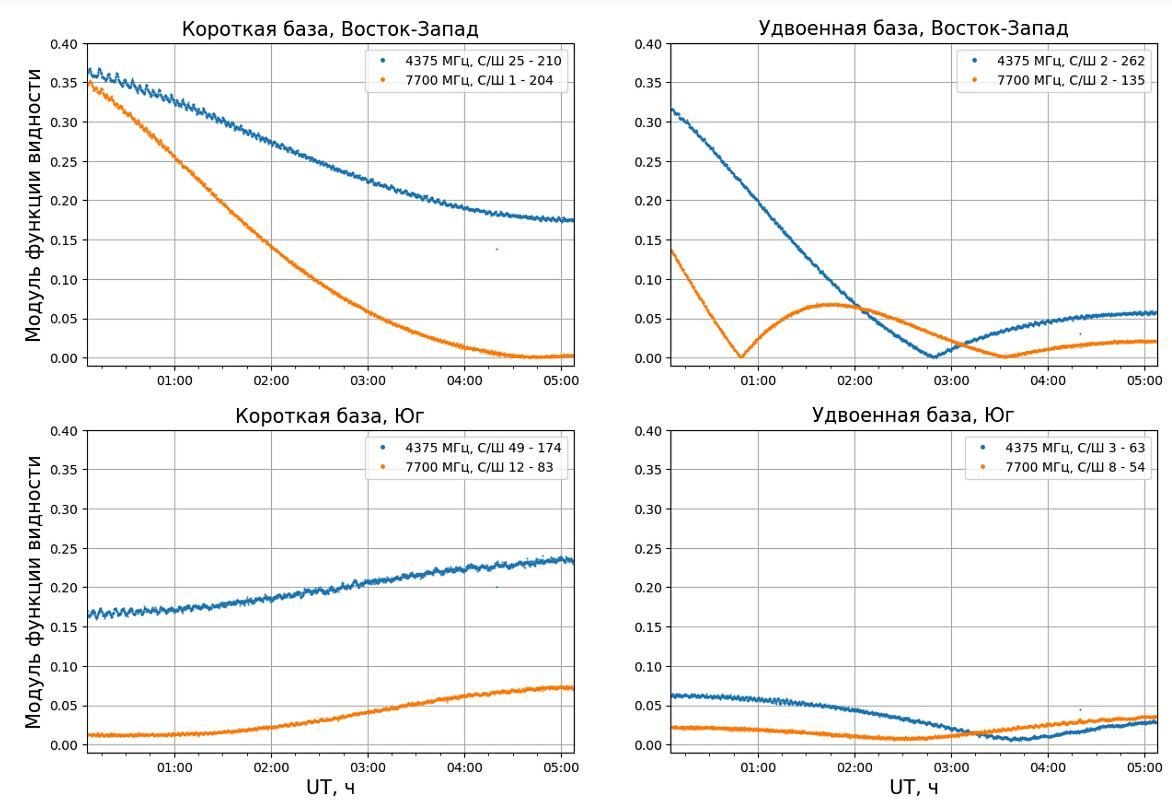
\includegraphics[scale=1]{images/SNRonbase.jpg}
	\caption{Изменение SNR на базах в течение дня}
	\label{fig:SNRonbase}
\end{figure}

На изображениях Солнца отсутствие и наличие фазовой калибровки выглядит, как представлено на рис. \ref{fig:notcalibandcalib}

\begin{figure}[H]
	\centering
	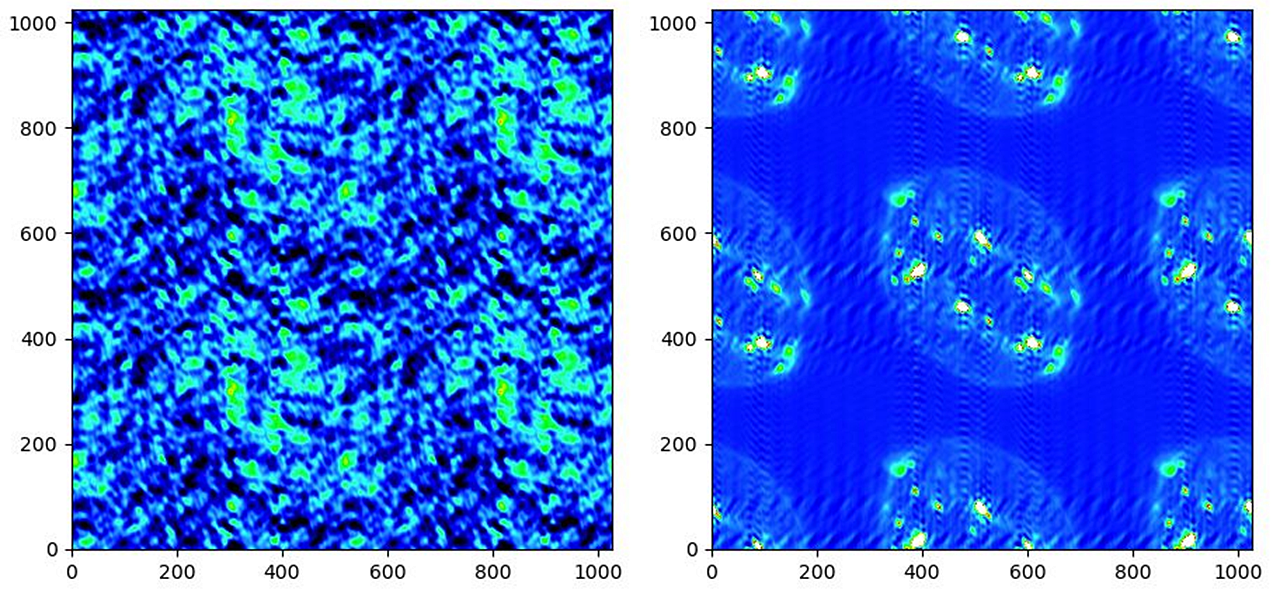
\includegraphics[width=1\linewidth]{images/notcalib_and_calib}
	\caption{Радиоизображение Солнца без фазовой калибровки и при ее наличии}
	\label{fig:notcalibandcalib}
\end{figure}

Также положительное влияние фазовой калибровки хорошо заметно и на $UV$-плоскости (рис. \ref{fig:UV_notcalibandcalib}).

\begin{figure}[H]
	\centering
	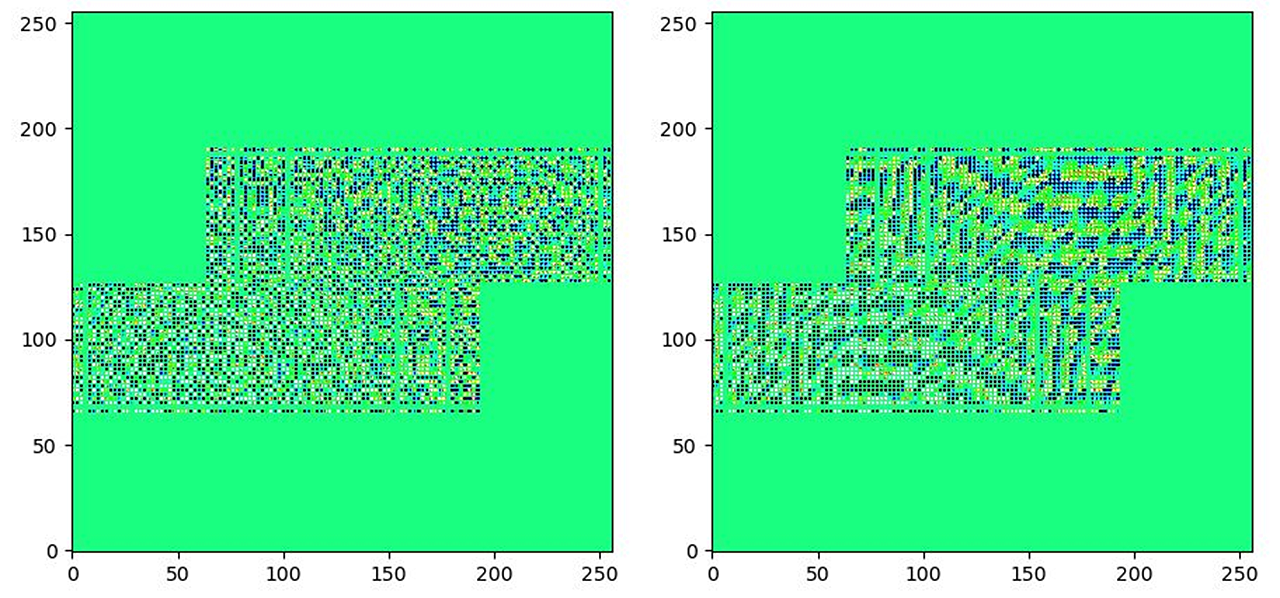
\includegraphics[width=1\linewidth]{images/UV_notcalib_and_calib}
	\caption{Фазовый портрет на $UV$-плоскости без фазовой калибровки и при ее наличии}
	\label{fig:UV_notcalibandcalib}
\end{figure}

\begin{figure}[H]
	\centering
	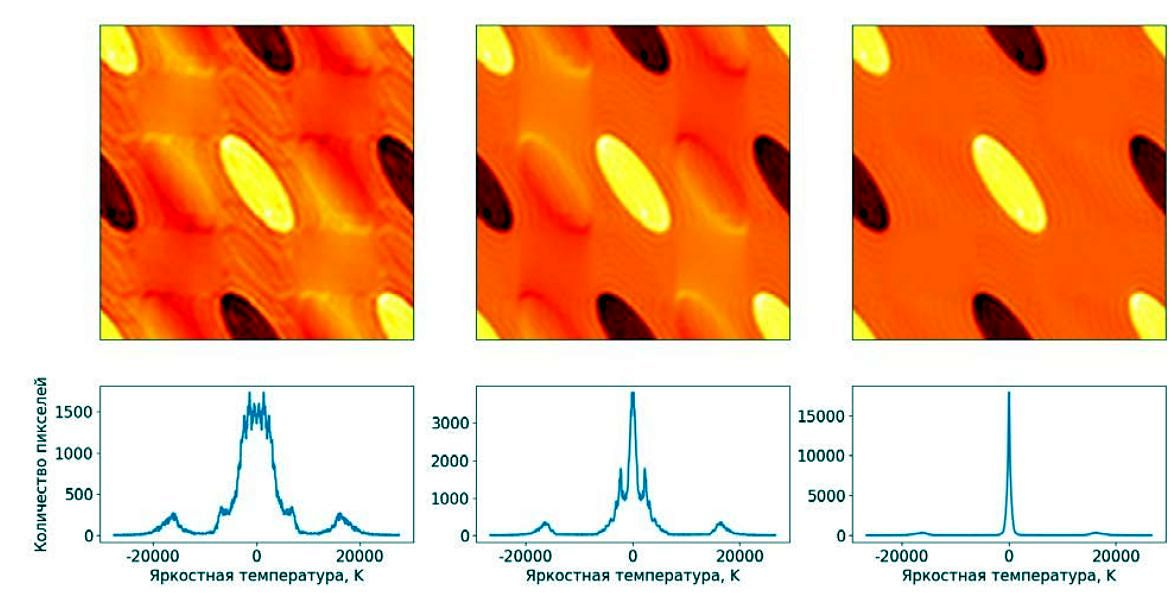
\includegraphics[width=1\linewidth]{images/temp_calib}
	\caption{Влияние амплитудной калибровки на изображения}
	\label{fig:temp_calib}
\end{figure}

На рис. \ref{fig:temp_calib} показано влияние амплитудной калибровки на получающееся изображение. Видно наличие артефактов и размытие гистограммы распределения яркостной температуры на левой (сопутствует калибровке только по коротким базам) и центральной (сопутствует калибровке и по длинным базам) картинках. Правая картинка соответствует хорошей фазовой и амплитудной калибровкам.

\begin{figure}[H]
	\centering
	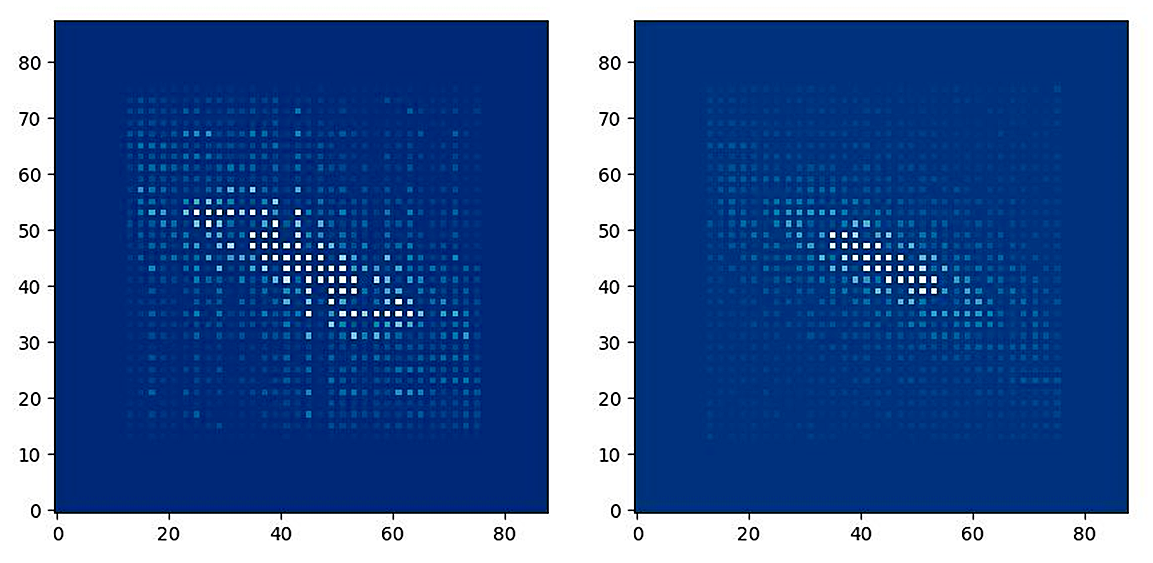
\includegraphics[width=1\linewidth]{images/amplitude_notcalib_and_calib}
	\caption{Влияние амплитудной калибровки на фазовую плоскость}
	\label{fig:amplitude_notcalib_and_calib}
\end{figure}

\noindent\textit{Подробнее о методе калибровки по избыточности можно прочитать в работах \cite{Wieringa}, \cite{Liu}}

\subsection{Корректировка остаточных эффектов}
После проведения калибровки необходимо произвести привязку яркостных температур и выполнить центрирование солнечного диска.

\subsubsection{Привязка температур}
Задача -- для каждой антенны перейти к антенной температуре и потокам. Существует два метода выполнения этой процедуры.

Первый заключается в анализе гистограммы распределения радиояркости на изображении \cite{trees}. Так как большую часть изображения занимает солнечный диск, можно сказать, что максимумом гистограммы является полученная яркостная температура спокойного Солнца. Зная "<эталонную"> температуру на разных частотах, в частности, из работы \cite{Zirin}, можно внести корректировки в изображение, домножив его на некоторый коэффициент и тем самым сместив максимум гистограммы.

Второй метод состоит в абсолютной привязке температур к известной величине.

Пусть на небе существует объект с яркостной температурой $T_B$, сигнал от которого принимает антенна c эффективной площадью $A_{eff}$.\\
Привяжем мощностную характеристику к некоторой $T_A$
\begin{equation}\label{eq:антенная температура}
	T_A = \dfrac{1}{\lambda^2} \int_{4 \pi}^{} A_{eff} T_B (\Omega) d\Omega
\end{equation}
Эту формулу можно оценивать как нормированный отклик антенны, умноженный на некоторую эффективную площадь. В случае, если $T_B$ постоянна для всей замкнутой поверхности вокруг антенны (случай безэховой камеры), то можно вынести ее из под знака интеграла как константу, и антенная температура окажется равной яркостной:
\begin{equation}\label{eq:равность температур}
	T_A = T_B
\end{equation}
Это позволит получать значения в единицах плотности потока ($SFU$):
\begin{equation}\label{eq:перевод в плотность потока}
	S_V = \dfrac{2kT_A}{\lambda^2} \Omega
\end{equation}

Однако для интерферометра нет безэховой камеры, а поток излучения от Солнца постоянно меняется.

Луна -- один из источников, который можно использовать для привязок из-за ее стабильности: поток меняется в пределах $10\%$ в зависимости от ее фазы. Однако до конца не ясно, как должен выглядеть спектр Луны в диапазоне наблюдений СРГ (3-24 ГГц).

Также стоит учитывать уровень сигнала и необходимую для его принятия чувствительность. Яркостная температура Луны -- около $200~K$, антенная температура СРГ при этом составит всего около $20~K$. Кроме того, влияет поглощение в атмосфере (особенно, когда точка наблюдений близка к горизонту) и погода (облачность) - снижение уровня принимаемого излучения может быть сопоставимо или даже превышать $20~K$. Антенная температура же при наблюдениях Солнца -- $1500$-$2000~K$.

\begin{figure}[H]
	\centering
	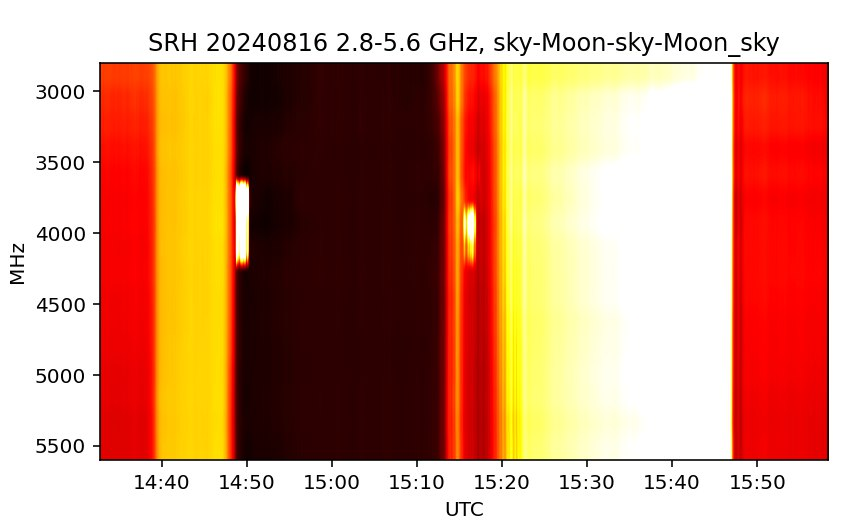
\includegraphics[width=0.7\linewidth]{images/moon_spectre}
	\caption{Спектрограмма наблюдений Луны с перерывами на наблюдения неба}
	\label{fig:moon_spectre}
\end{figure}

\begin{figure}[H]
	\centering
	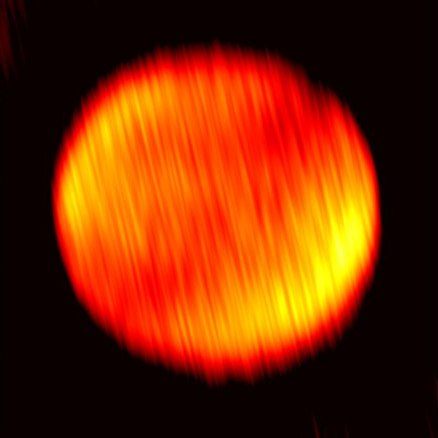
\includegraphics[width=0.7\linewidth]{images/moon_radio}
	\caption{Изображение Луны в радиодиапазоне, сумма нескольких частот, макс. 4.8 ГГц}
	\label{fig:moon_radio}
\end{figure}

На некоторых радиотелескопах для этих целей используется искусственная Луна (например, на Карадагском полигоне в Крыму) - большой черный диск на некотором расстоянии от интерферометра.\\ На СРГ для калибровки используется лес, постольку поскольку он, во первых, является довольно стабильным источником, а во вторых, с помощью него можно создать некий эквивалент безэховой камеры. Это осуществимо потому, что главный лепесток антенн можно полностью закрыть этим лесом. Зная ширину диаграммы направленности, температуру леса, которая примерно равна температуре окружающей среды и частоту наблюдений также можно рассчитать и внести соответствующие корректировки.\\
Каждая сессия ежедневных наблюдений оканчивается наведением антенн на лесной массив вблизи обсерватории.

Таким образом, алгоритм привязки яркостной температуры на данный момент таков: ежедневно подбирается такая зависимость оптической толщины леса в диапазоне частот наблюдений СРГ, чтобы  калибровка по потокам совпала с данными Нобеямского спектрополяриметра -- пока проводится подгонка для разных времен года.

В данный момент рассматривается идея с экранированием облучателя антенны радиопоглощающим материалом, с целью определения оптической толщины леса.

\subsubsection{Привязка координат}
Существуют различные алгоритмы поиска окружностей на изображении, однако здесь невозможно их использовать из-за наложений вторичных солнечных дисков.

В пакете \texttt{srhdata} для центрирования диска строится модельный диск Солнца, который затем сворачивается с диаграммой направленности интерферометра, и уже полученная функция соотносится с результатом наблюдений, который и подгоняется под модель.

Возможно выполнять выравнивание, опираясь на данные наблюдений в других диапазонах, используя пятна и стабильные микроволновые источники над ними. Данный метод позволяет соотнести изображения более точно, но также имеет свои недочеты, в частности, пятенные источники обычно пропадают на частотах 13-15 ГГц, и выше этих значений уже не наблюдаются.


\subsection{Как калибровать?}
Математически задачу калибровки можно описать так. Пусть у нас есть некоторое выражение
\begin{equation}\label{eq:видности}
	\widetilde{V}_{kl}(t) = g_k(t)g_l^*(t)G_{kl}(t)V_{kl}(t) + \epsilon_{kl}(t) + \varepsilon_{kl}(t)
\end{equation}
где:
\begin{list}{-}{}
	\item $\widetilde{V}_{kl}(t)$ -- измеренная видность
	\item  $V_{kl}$ -- истинная видность, то есть компонента пространственного спектра функции, из которой мы можем построить изображение (иначе говоря, Фурье-компонента пространственного спектра распределения яркости, соответствующая базе).
\end{list}
Остальные параметры выражения имеют аппаратное происхождение, а именно:
\begin{list}{-}{}
	\item $g_k(t)$ и $g_l^*(t)$ -- коэффициенты передачи $k$-ой и $l$-ой антенны ($l$ - сопряженная антенна)
	\item $\varepsilon_{kl}(t)$ -- температурные шумы
	\item $G_{kl}(t)$ -- ошибки, связанные с конкретной базой
	\item $\epsilon_{kl}(t)$ -- аддитивная постоянная составляющая для пары антенн (например, ошибки коррелятора - подобное можно отследить)
\end{list}

От ошибок $G_{kl}(t)$ и $\varepsilon_{kl}(t)$ стараются всегда избавиться инструментально. Получать эти ошибки из системы уравнений - очень трудоёмкая задача, т.к. их нельзя разложить на отдельные множители, связанные с антеннами.

Таким образом, суть калибровки можно свести к определению истинных видностей $V_{kl}(t)$ путем поиска и учета паразитных членов в правой части выражения \eqref{eq:видности}.

Радиотелескопы апертурного синтеза в общем случае нельзя скалибровать раз и навсегда из-за:
\begin{itemize}
	\item недостаточной точности позиционирования антенн (возникают	дополнительные набеги фаз, зависящие от координат источника на небесной сфере)
	\item не идентичной конструкции антенн (плохое наведение отдельных антенн, их различные передаточные характеристики)
	\item влияния температуры и характеристик окружающей среды на параметры приемного тракта антенны
	\item влияния атмосферы (дополнительный набег фаз из-за разной толщи атмосферы, через которую проходит излучение)
\end{itemize}

\subsection{Пространственные гармоники}
Каждая пара антенн измеряет свою пространственную гармонику, которая в свою очередь является очень сложной функцией переменной частоты (зависит от проекции базы) и опирается значение функции Бесселя (диаграмма направленности одиночной антенны). Пространственные гармоники в пределах малых углов можно интерпретировать как идеальные двумерные гармоники и использовать для их расчета обычный Фурье-анализ.

При этом пространственная частота и ориентация гармоники определяются вектором базы и частотой приема (см. короткую "<низкочастотную"> и длинную "<высокочастотную"> базы на рис. \ref{fig:гармоники}): чем больше база, тем выше частота и тем менее протяженные объекты можно обнаружить.

\begin{figure}[H]
	\centering
	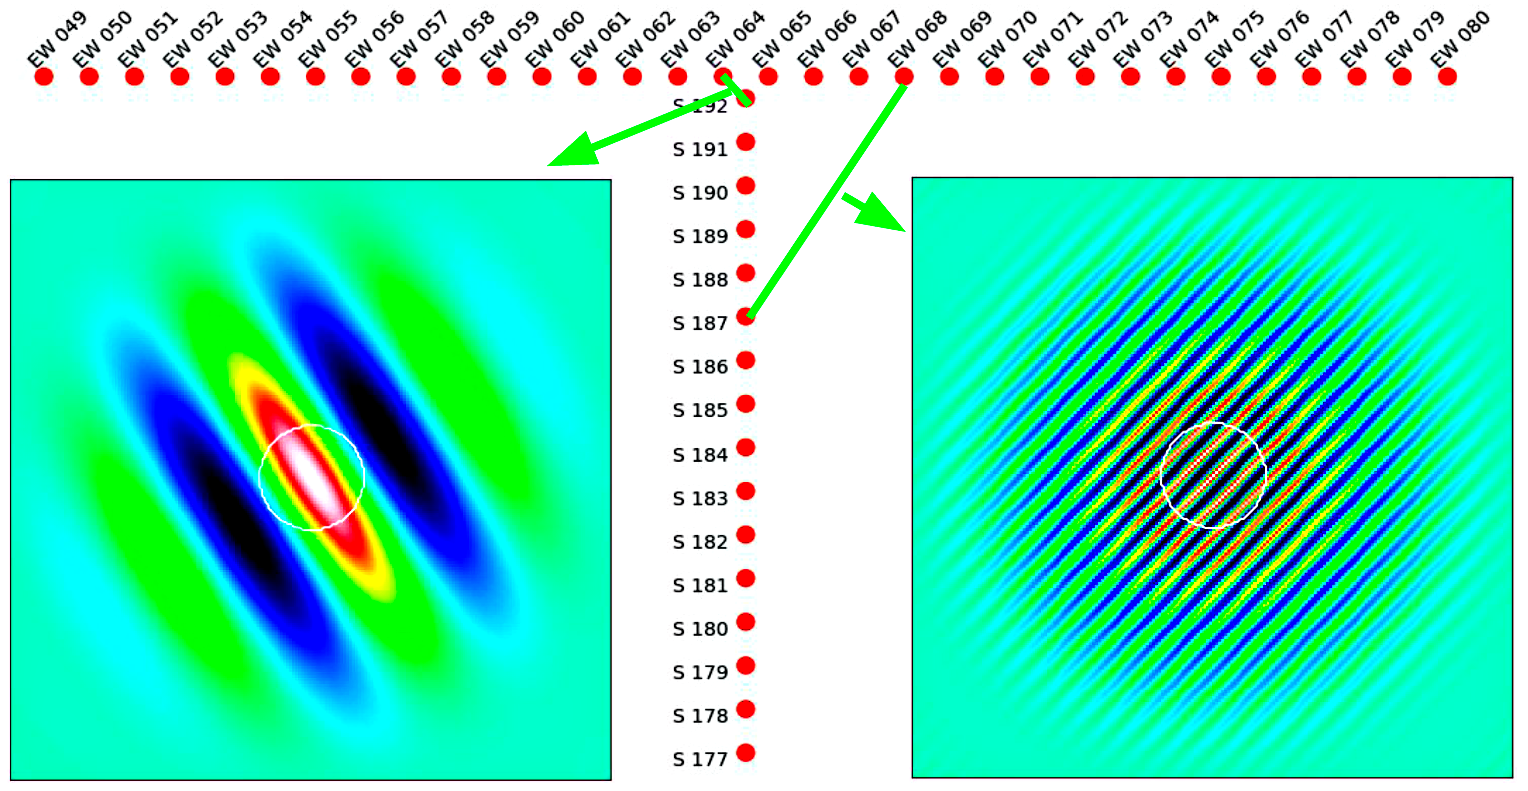
\includegraphics[scale=0.43]{images/globa1.png}
	\caption{Измерение парами антенн пространственных гармоник}
	\label{fig:гармоники}
\end{figure}

$UV$-плоскость формируется путем комбинирования результатов измерений пространственных гармоник каждой антенной пары. $UV$-плоскость позволяет визуализировать пространственную информацию о наблюдаемом объекте с высоким разрешением. Обработка данных в $UV$-плоскости обеспечивает возможность нахождения деталей и структур объектов, а также их спектральных характеристик.

\section{Построение изображений Сибирского Радиогелиографа}
\subsection{Заполнение $UV$-плоскости}
СРГ представляет собой комплекс из трех антенных решеток:
\begin{itemize}
	\item 3-6 ГГЦ: 129 антенн диаметром 3 метра с эквидистантной расстановкой в 9.8 метра, восточный, западный и северный лучи -- первый длиннее остальных, что приводит к несимметричной $UV$-плоскости
	\item 6-12 ГГЦ: 192 антенн диаметром 2 метра с эквидистантной расстановкой в 4.9 метра, каждый луч имеет 64 антенны, но нет связующей антенны между лучами
	\item 12-24 ГГЦ: 207 антенн диаметром 1 метр с неэквидистантным расположением -- центральный сектор имеет плотное расположение, далее шаг увеличивается в 2 раза, еще дальше - в 4 раза от первоначальной величины в \textcolor{red}{2.45} метра. Сделано это для увеличения пространственного разрешения
\end{itemize}

\begin{figure}[H]
	\centering
	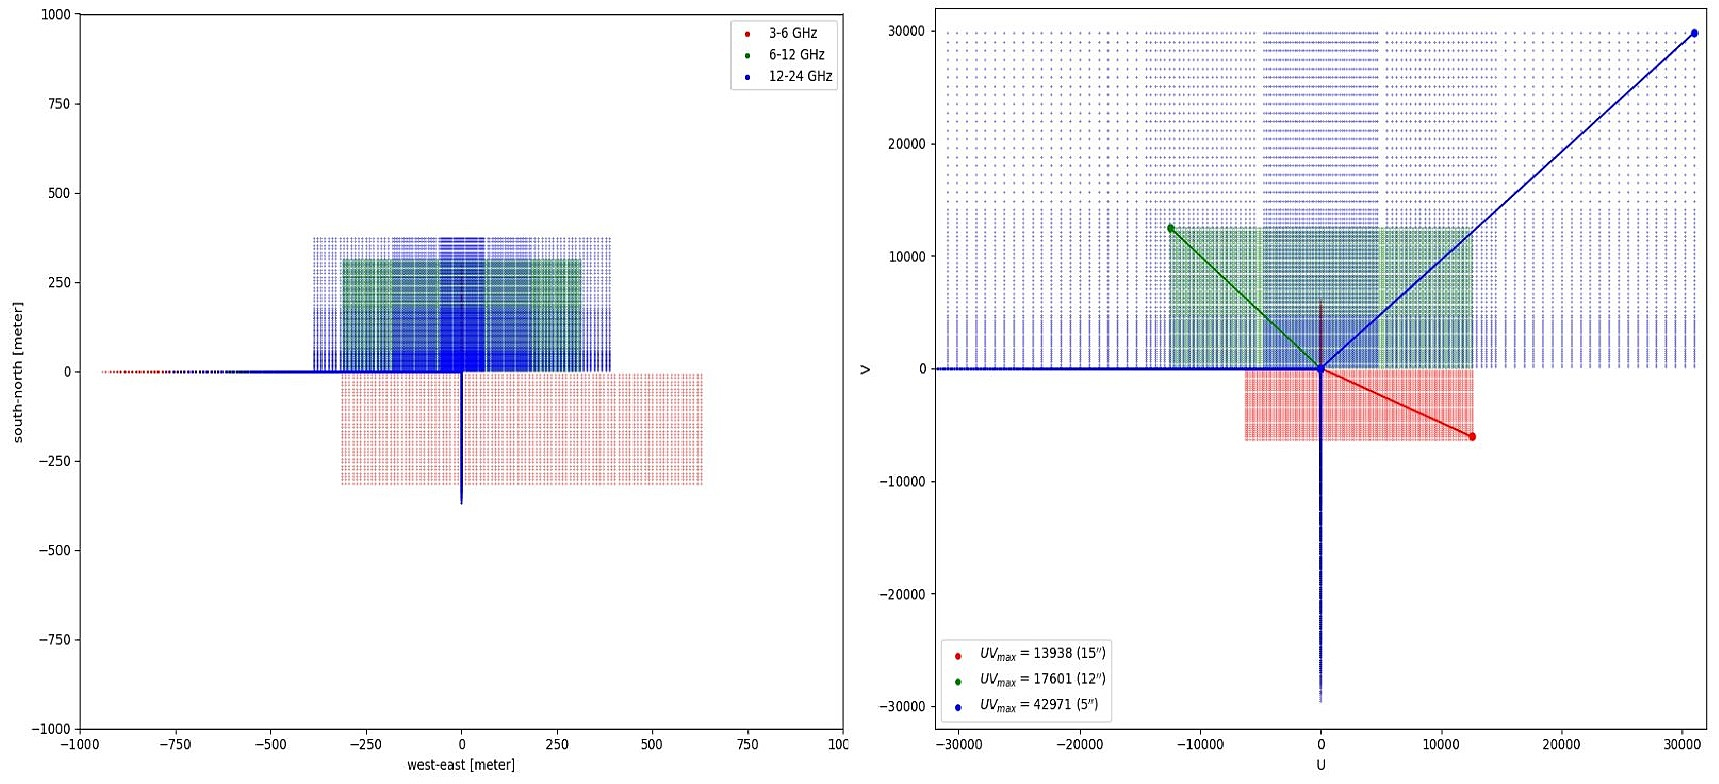
\includegraphics[scale=0.28]{images/srh_UV}
	\caption{Заполнение $UV$-плоскости антеннами различных диапазонов: отображение в метрах (слева) и пространственных частотах (справа). Красным обозначена решетка 3-6 ГГц, зеленым -- 6-12 ГГц, синим -- 12-24 ГГц}
	\label{fig:srh_UV}
\end{figure}

На рис. \ref{fig:srh_UV} представлены $UV$-плоскости для различных антенных решеток СРГ, причем отображены как перекрестные базы, так и избыточные базы, образуемые антеннами на одном луче. Как видно по левой части изображения, где $UV$-плоскость отображена в метрах, на решетке 3-6 ГГц линия с этими избыточными базами выходит наиболее далеко -- это объясняется наибольшей длиной луча этой решетки, равной 900-ам метрам. Также видно и неравномерное покрытие решетки 12-24 ГГц.

Полоски, тянущиеся на \ref{fig:srh_UV}, определяют максимальное пространственное разрешение. Можно увидеть, насколько возможное разрешение решетки 12-24 ГГц превышает остальные две -- это является следствием неэквидистантного раположения антенн.

\begin{figure}[H]
	\centering
	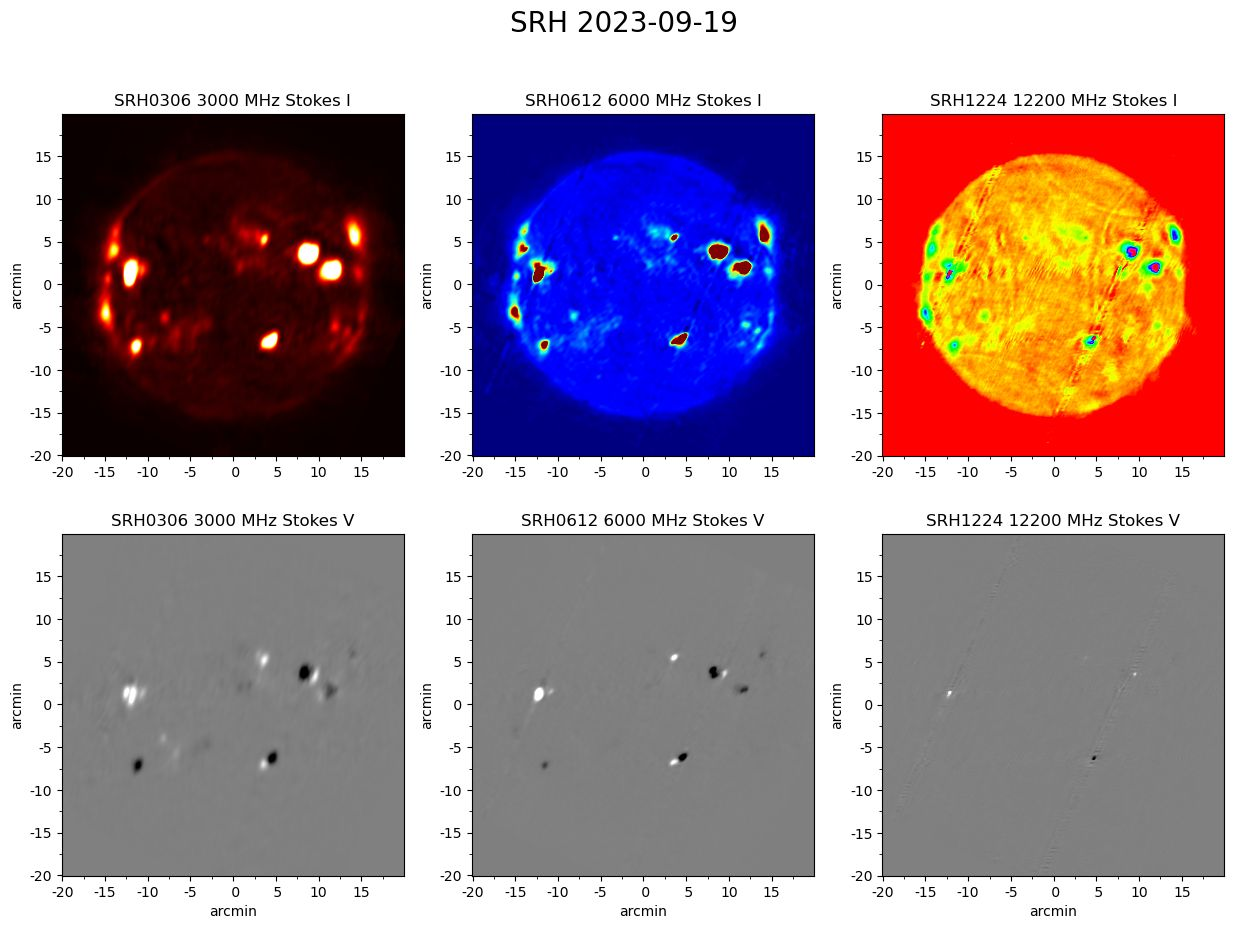
\includegraphics[scale=0.9]{images/img_example}
	\caption{Примеры изображений с разных решеток интерферометра: сверху представлена суммарная интенсивность правой и левой круговой поляризаций $I$, снизу -- их разность, параметр Стокса $V$}
	\label{fig:img_example}
\end{figure}

Как можно заметить из рис. \ref{fig:img_example}, на изображениях диапазона 12-24 ГГц имеются полосы -- подобный эффект наблюдается также и на данных наблюдений Нобеямского радиогелиографа, и является следствием неравномерного заполнения $UV$-плоскости.

\begin{figure}[H]
	\centering
	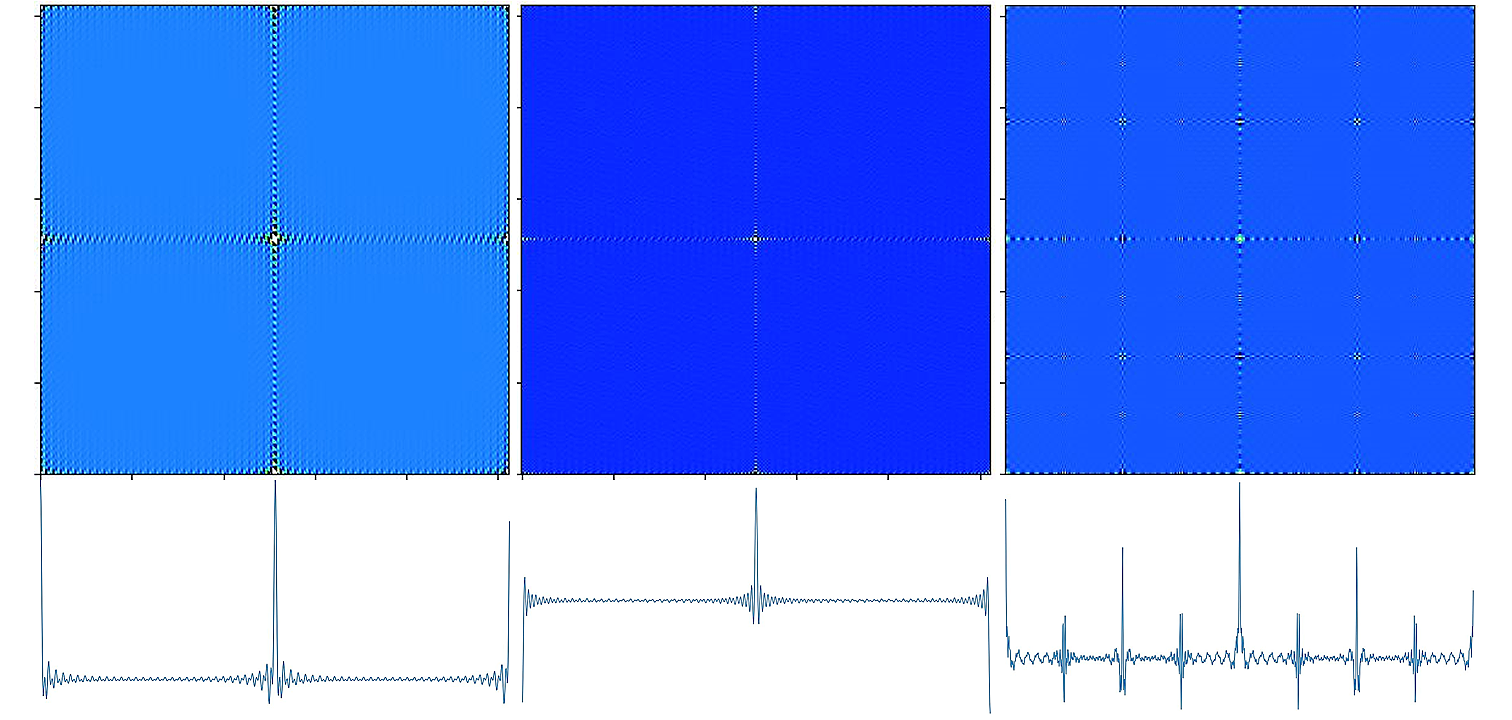
\includegraphics[scale=0.43]{images/psfs}
	\caption{Диаграммы направленности решеток интерферометра в системе координат направляющих косинусов}
	\label{fig:psfs}
\end{figure}

Из рисунка \ref{fig:psfs} видно, что вторичные максимумы диаграммы направленности для решеток 3-6 и 12-24 ГГц имеют положительный знак, а для решетки 6-12 ГГц -- отрицательный. Также видно еще одно следствие несимметричности лучей решетки 3-6 ГГц -- нерегулярная структура ее лепестков, а также следствие неэквидистантности антенн решетки 12-24 -- сложная структура ее диаграммы направленности, с дополнительными знакопеременными лепестками, от которых потом довольно сложно очищать изображение.

\subsection{Теорема Ван Циттерта-Цернике}
Основная теорема интеферометрии звучит так:
\newtheorem*{Van_Cittert_Zernike}{Теорема Ван Циттерта-Цернике}
\begin{Van_Cittert_Zernike}
Распределение интенсивности по углу связано с взаимной когерентностью падающего излучения через преобразование Фурье, т.е.:
\begin{equation}\label{eq:Ван Циттерт-Церник}
	\Gamma_{12} (u,v,0) = \iint I(l,m) e^{-2\pi i(ul+vm)} dl \, dm
\end{equation}
\end{Van_Cittert_Zernike}
\noindent $u$ и $v$ в формуле \ref{eq:Ван Циттерт-Церник} являются пространственными частотами, $l$ и $m$ -- направляющие косинусы. Эта система координат удобна, потому как в ней $UV$-плоскость и диаграмма направленности выглядят одинаково, а меняется только форма и размер источника.

\begin{figure}[H]
	\centering
	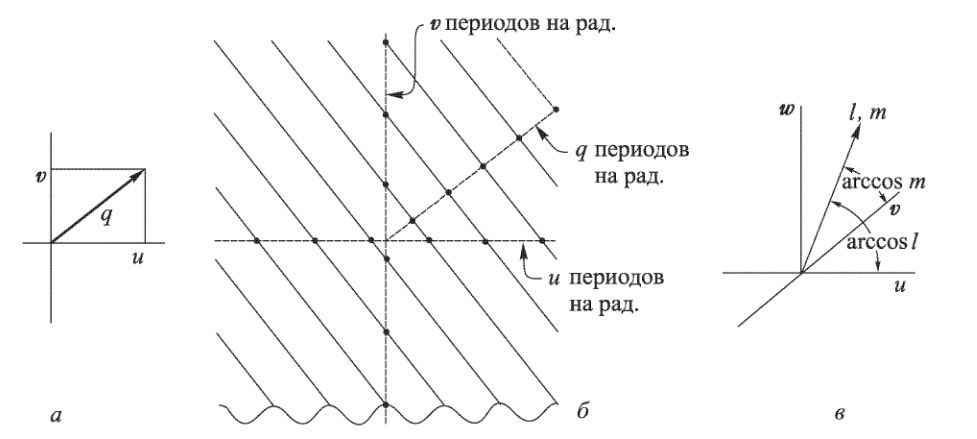
\includegraphics[scale=0.8]{images/cosinuses}
	\caption{К объяснению системы координат направляющих косинусов}
	\label{fig:cosinuses}
\end{figure}

Функция взаимной когерентности в данном случае определяется перемножением сигналов с пар антенн, произведение которых затем усредняется. В свою очередь, сигнал определяется видностями, которые связаны с распределением радиояркости на небе через преобразование Фурье (рис. \ref{fig:Van_Cittert_Zernike}).

\begin{figure}[H]
	\centering
	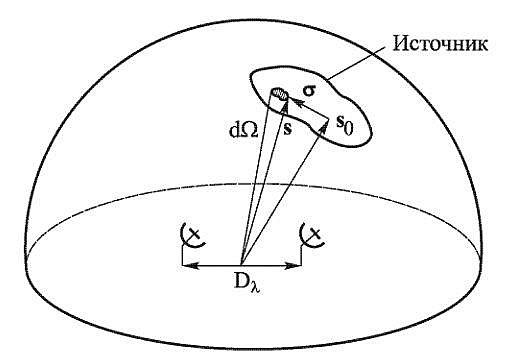
\includegraphics[scale=1]{images/Van_Cittert_Zernike}
	\caption{Схематическое пояснение теоремы Ван Циттерта-Цернике}
	\label{fig:Van_Cittert_Zernike}
\end{figure}

\subsection{Преобразование Фурье и теорема о свертке}
Пусть есть $a(t)$, $b(t)$, тогда
\begin{equation}\label{eq:Фурье А}
	A(\omega) =\int_{-\infty}^{\infty} a(t)exp(i \omega t) dt,
\end{equation}
\begin{equation}\label{eq:Фурье В}
	B(\omega) =\int_{-\infty}^{\infty} b(t)exp(i \omega t) dt
\end{equation}
-- Фурье-образы функций $a(t)$, $b(t)$.

\newtheorem*{Convolution_theorem}{Теорема о свёртке}
\begin{Convolution_theorem}
	Перемножение сигналов по времени равносильно сворачиванию их спектров, и наоборот
\end{Convolution_theorem}

Таким образом:
\begin{equation}\label{eq:ThConvolution1}
	a(t) \cdot b(t) = A(\omega) * B(\omega),
\end{equation}
\begin{equation}\label{eq:ThConvolution2}
	a(t) * b(t) = A(\omega) \cdot B(\omega)
\end{equation}

Операция же свертки представляет собой следующую процедуру:
\begin{equation}\label{eq:Convolution}
	(f * g)(t) := \int_{-\infty}^{\infty} f(\tau) g(t-\tau) d\tau
\end{equation}

\begin{figure}[H]
	\centering
	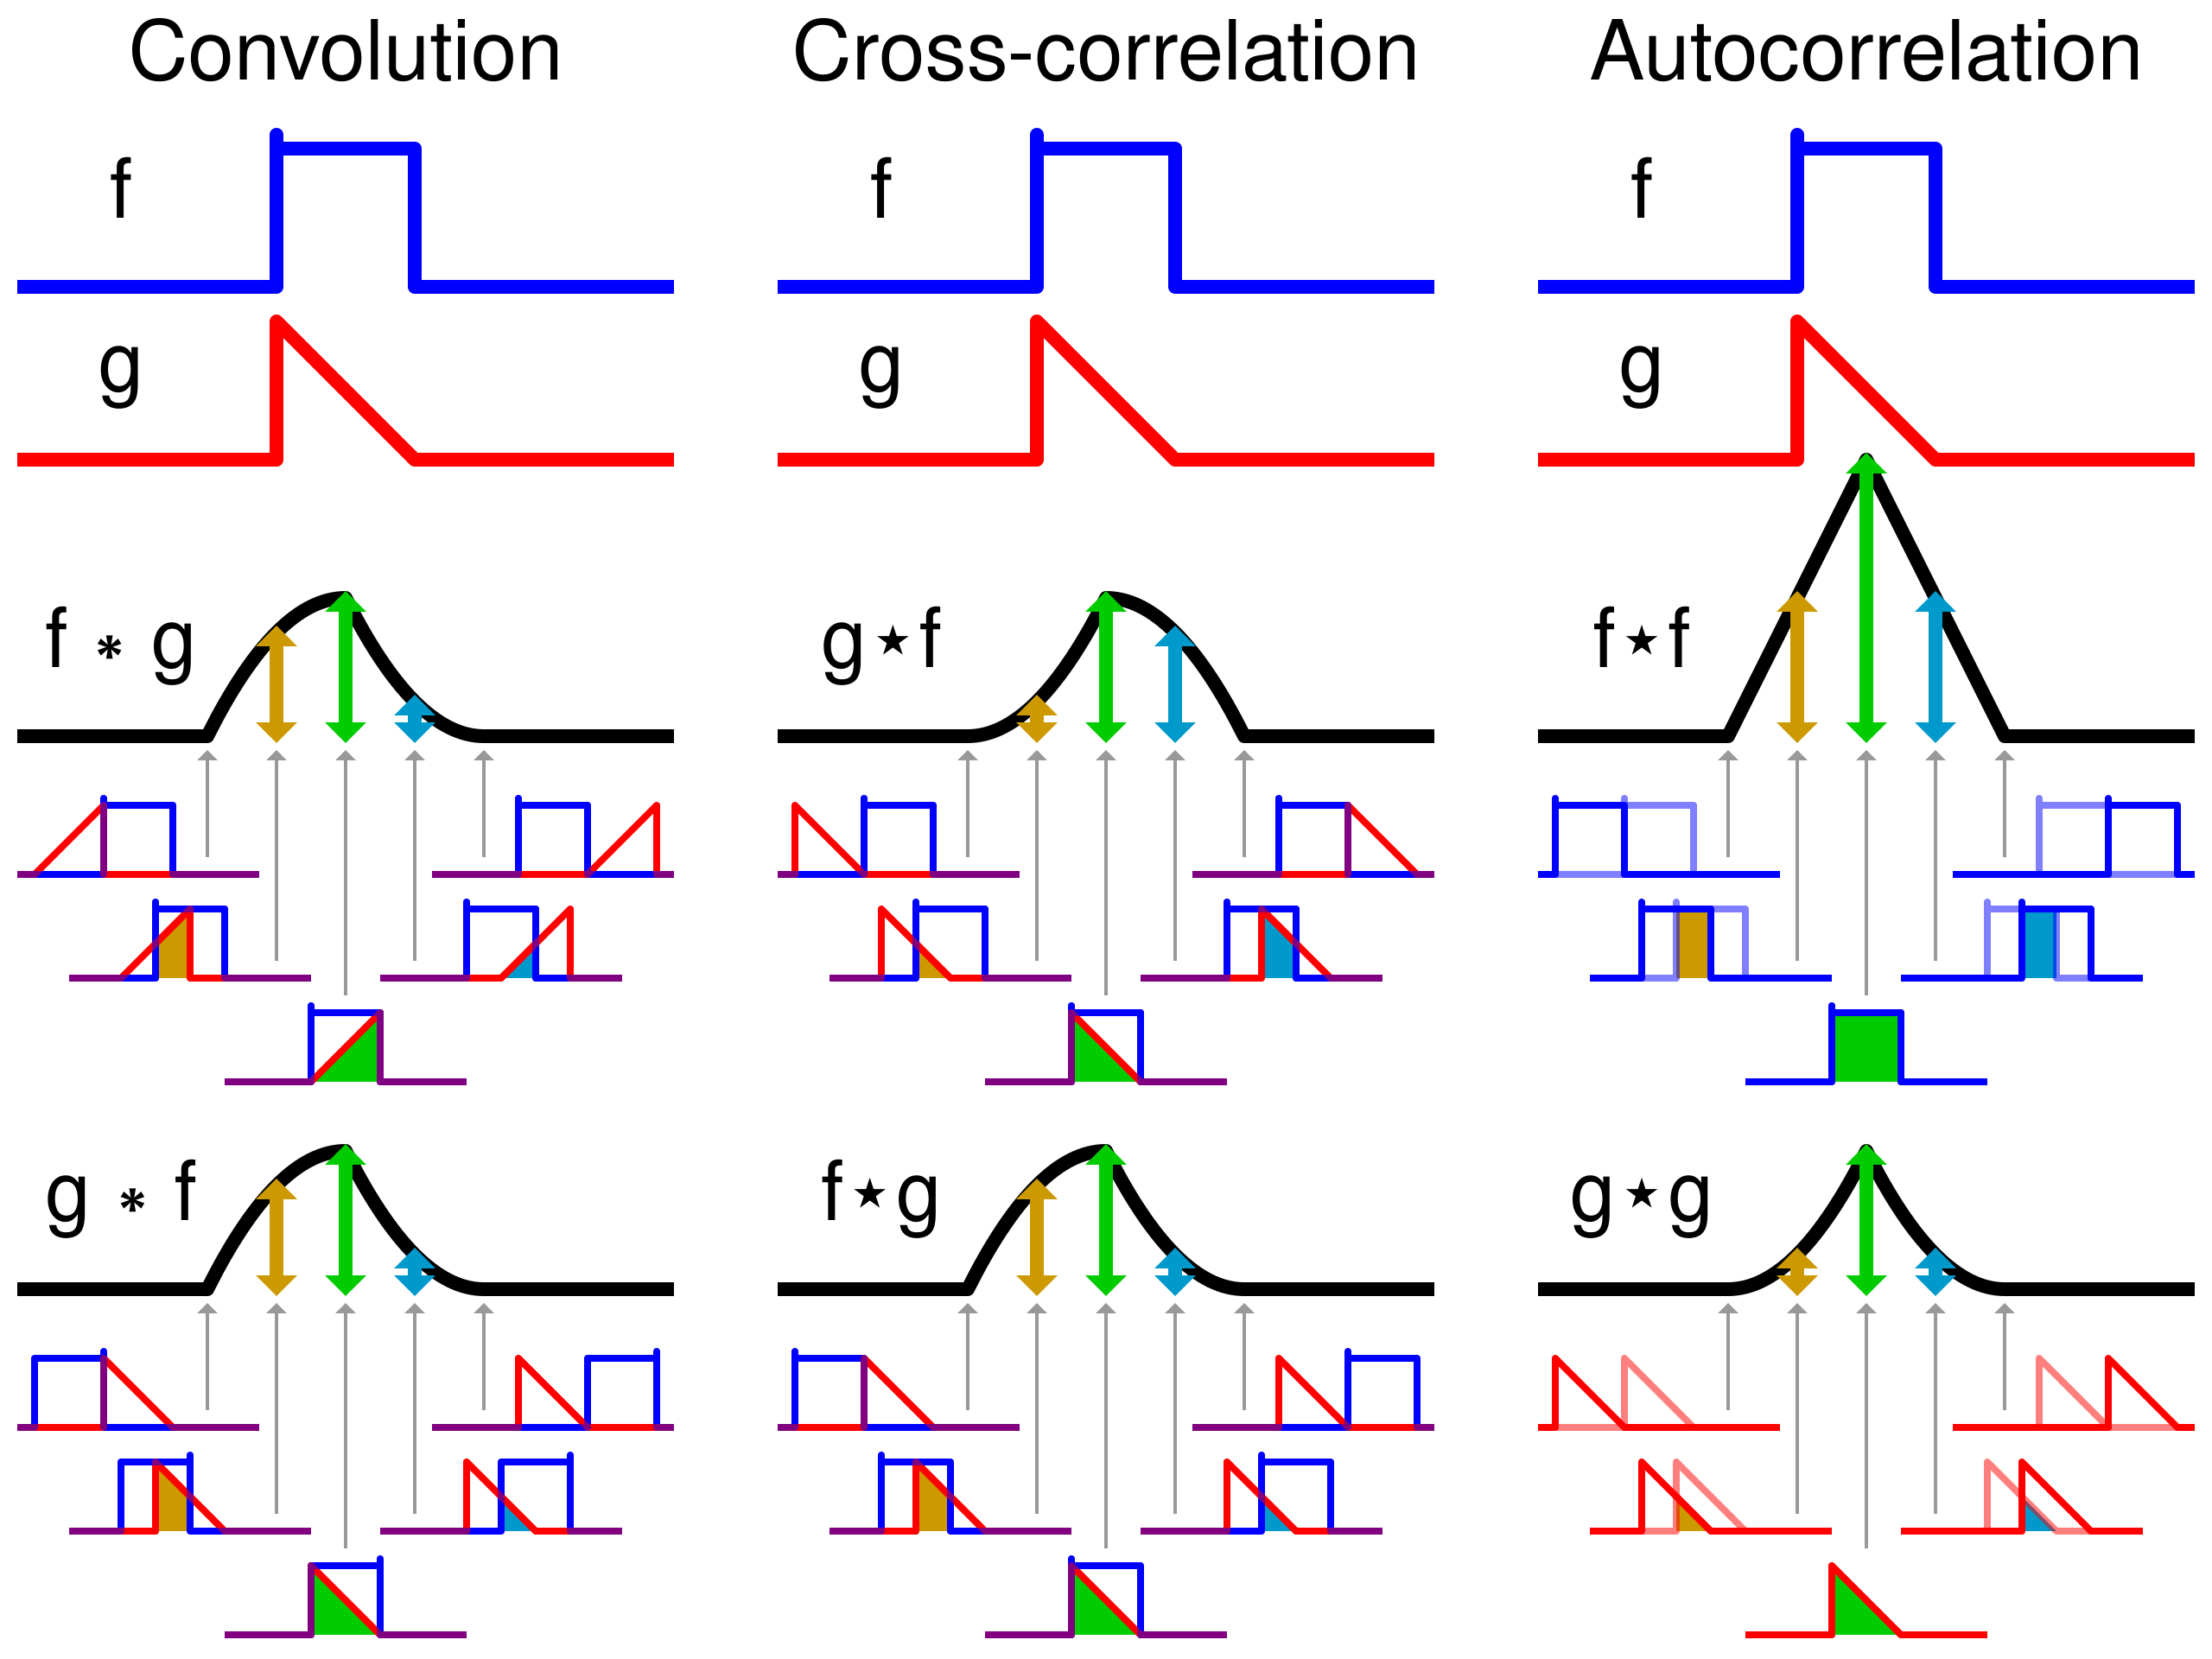
\includegraphics[scale=0.14]{images/Comparison_convolution_correlation}
	\caption{Визуальное сравнение свертки, взаимной корреляции и автокорреляции}
	\label{fig:Comparison_convolution_correlation}
\end{figure}

\noindent Функция, с которой происходит сворачивание, называется ядром свертки.

\begin{figure}[H]
	\centering
	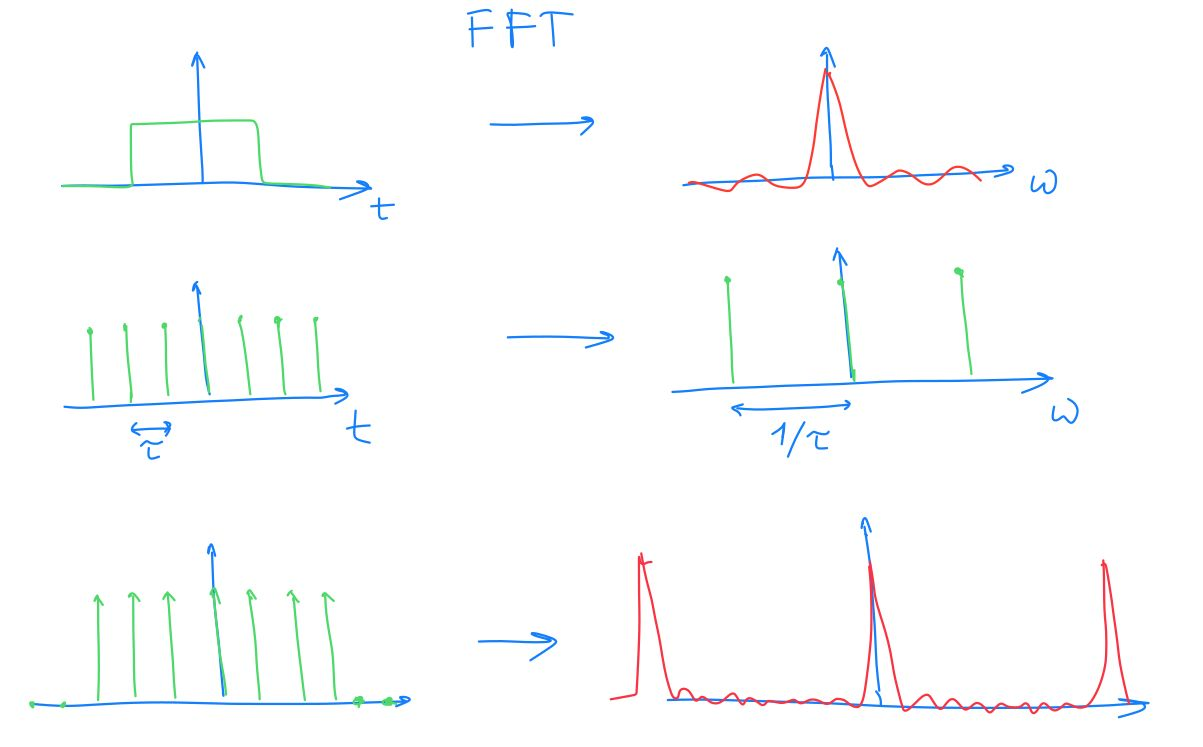
\includegraphics[scale=0.8]{images/FFT1}
	\caption{Пары сигнал - спектр}
	\label{fig:FFT1}
\end{figure}

\begin{figure}[H]
	\centering
	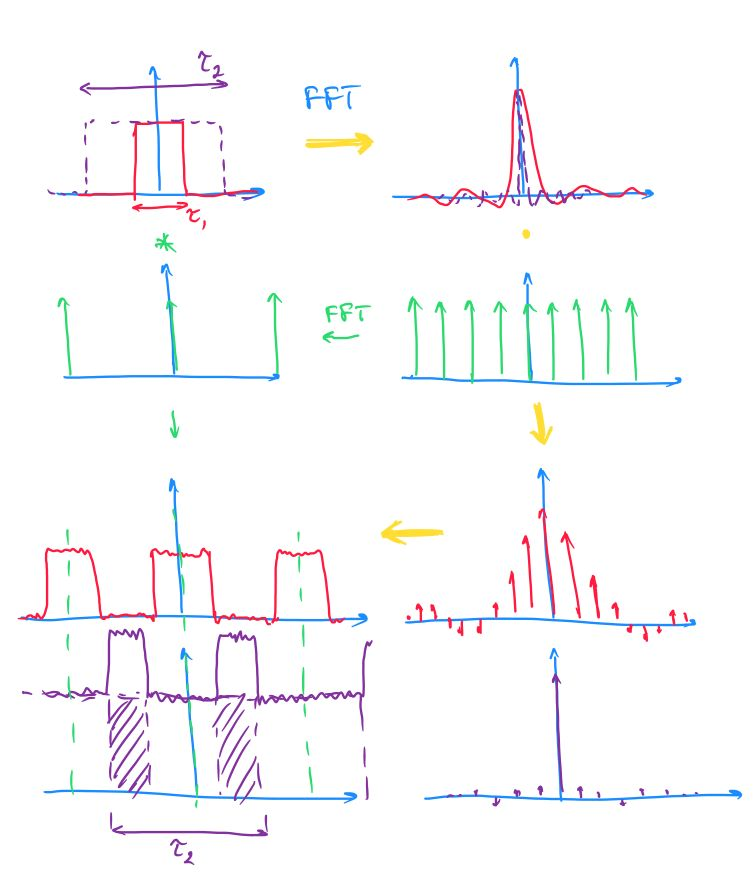
\includegraphics[scale=0.8]{images/FFT2}
	\caption{Пары сигнал - спектр}
	\label{fig:FFT2}
\end{figure}

\section{Введение}

\begin{figure}[H]
	\centering
	
\includegraphics[scale=0.55]{img/smile.png}
	\caption{гыгыгыгыгыгыгыгыгы}
	\label{fig:gygygy}
\end{figure}

Это шаблон учебного пособия, в котором можно показывать рисунки (см. рис. \ref{fig:gygygy})

\subsection{Делать подразделы}
Вот

\paragraph{Еще и параграфы}
И ссылаться на литературу \cite{priest}

